\section{eo\-Det\-Bit\-Flip$<$ Chrom $>$ Class Template Reference}
\label{classeo_det_bit_flip}\index{eoDetBitFlip@{eoDetBitFlip}}
eo\-Det\-Bit\-Flip --$>$ changes exactly k bits  


{\tt \#include $<$ga/eo\-Bit\-Op.h$>$}

Inheritance diagram for eo\-Det\-Bit\-Flip$<$ Chrom $>$::\begin{figure}[H]
\begin{center}
\leavevmode
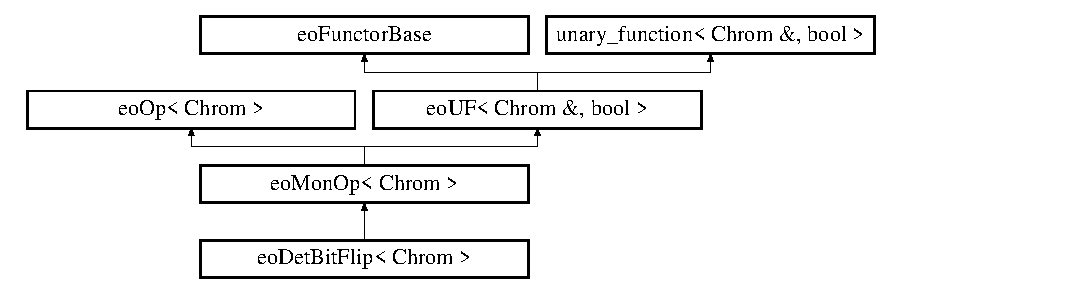
\includegraphics[height=3.50548cm]{classeo_det_bit_flip}
\end{center}
\end{figure}
\subsection*{Public Member Functions}
\begin{CompactItemize}
\item 
{\bf eo\-Det\-Bit\-Flip} (const unsigned \&\_\-num\_\-bit=1)
\begin{CompactList}\small\item\em (Default) Constructor. \item\end{CompactList}\item 
virtual std::string {\bf class\-Name} () const \label{classeo_det_bit_flip_a1}

\begin{CompactList}\small\item\em The class name. \item\end{CompactList}\item 
bool {\bf operator()} (Chrom \&chrom)
\begin{CompactList}\small\item\em Change num\_\-bit bits. \item\end{CompactList}\end{CompactItemize}
\subsection*{Private Attributes}
\begin{CompactItemize}
\item 
unsigned {\bf num\_\-bit}\label{classeo_det_bit_flip_r0}

\end{CompactItemize}


\subsection{Detailed Description}
\subsubsection*{template$<$class Chrom$>$ class eo\-Det\-Bit\-Flip$<$ Chrom $>$}

eo\-Det\-Bit\-Flip --$>$ changes exactly k bits 



Definition at line 67 of file eo\-Bit\-Op.h.

\subsection{Constructor \& Destructor Documentation}
\index{eoDetBitFlip@{eo\-Det\-Bit\-Flip}!eoDetBitFlip@{eoDetBitFlip}}
\index{eoDetBitFlip@{eoDetBitFlip}!eoDetBitFlip@{eo\-Det\-Bit\-Flip}}
\subsubsection{\setlength{\rightskip}{0pt plus 5cm}template$<$class Chrom$>$ {\bf eo\-Det\-Bit\-Flip}$<$ Chrom $>$::{\bf eo\-Det\-Bit\-Flip} (const unsigned \& {\em \_\-num\_\-bit} = {\tt 1})\hspace{0.3cm}{\tt  [inline]}}\label{classeo_det_bit_flip_a0}


(Default) Constructor. 

\begin{Desc}
\item[Parameters:]
\begin{description}
\item[{\em \_\-num\_\-bit}]The number of bits to change default is one - equivalent to eo\-One\-Bit\-Flip then \end{description}
\end{Desc}


Definition at line 75 of file eo\-Bit\-Op.h.

\subsection{Member Function Documentation}
\index{eoDetBitFlip@{eo\-Det\-Bit\-Flip}!operator()@{operator()}}
\index{operator()@{operator()}!eoDetBitFlip@{eo\-Det\-Bit\-Flip}}
\subsubsection{\setlength{\rightskip}{0pt plus 5cm}template$<$class Chrom$>$ bool {\bf eo\-Det\-Bit\-Flip}$<$ Chrom $>$::operator() (Chrom \& {\em chrom})\hspace{0.3cm}{\tt  [inline, virtual]}}\label{classeo_det_bit_flip_a2}


Change num\_\-bit bits. 

\begin{Desc}
\item[Parameters:]
\begin{description}
\item[{\em chrom}]The cromosome which one bit is going to be changed. \end{description}
\end{Desc}


Implements {\bf eo\-UF$<$ Chrom \&, bool $>$} {\rm (p.\,\pageref{classeo_u_f_a1})}.

Definition at line 84 of file eo\-Bit\-Op.h.

The documentation for this class was generated from the following file:\begin{CompactItemize}
\item 
eo\-Bit\-Op.h\end{CompactItemize}
